\documentclass[pdftex,cyrillic,14pt,a4page,twoside,openright]{extreport}
\usepackage[bulgarian]{babel}

\usepackage[margin=2cm]{geometry}% http://ctan.org/pkg/geometry
\usepackage[pdftex]{graphicx}
\usepackage{hyperref}
\graphicspath{ {./figures/} }

\usepackage{./titlesec/titlesec}

% Counter too wide line spacing added by twoside
% https://tex.stackexchange.com/questions/62572/twoside-introduces-incorrect-linespacing-at-end-of-section
\raggedbottom
  
\titleformat{\chapter}%
  {\normalfont\bfseries\Huge}{\thechapter.}{10pt}{}

\usepackage{afterpage}
\newcommand\blankpage{%
    \null
    \thispagestyle{empty}%
    \newpage}


\begin{document}
\begin{titlepage}
	\begin{center}
	
\includegraphics[scale=1.2]{./NBU_logo.jpg}\\[0.3cm]
    \textbf{\Large НОВ БЪЛГАРСКИ УНИВЕРСИТЕТ\\[0.4cm]}
    \textbf{\Large Департамент Информатика\\[0.4cm]}
    \textbf{\Large Бакалавърка програма Информатика\\[3cm]}
   
		\textbf{\LARGE Автоматизиран биоинформатичен анализ на генетични варианти, потенциално свързани със стареенето\\[2cm]}
		\begin{Large}
		Дипломна работа на\\[0.2cm]
		Михаил М. Здравков\\[3cm]
		\end{Large}
		\begin{minipage}{0.48\textwidth}
			\begin{flushleft} \large
				\emph{Научни ръководители:} \\
				доц. д-р Милена Георгиева \\
				Момчил Топалов
			\end{flushleft}
		\end{minipage}
			\begin{minipage}{0.48\textwidth}
			\begin{flushright} \large
				\emph{Дипломен консултант:} \\
				гл. ас. д-р Методи Трайков\\
				\clearpage
			\end{flushright}
		\end{minipage}

		\vfill

		% Bottom of the page
		{\large София 2022}

	\end{center}
\end{titlepage}


\afterpage{\blankpage}

\newgeometry{
	inner=30mm,
    outer=20mm,
    top=20mm,
    bottom=20mm}

\tableofcontents
\pagebreak
%\afterpage{\blankpage}

\setlength\parindent{0pt}

\chapter*{Използвани съкращения}
\textbf{HGVS} - Human Genome Variation Society. Организация, занимаваща се с генетични варианти при хората, дала името и на стандартна номенклатура за описване на варианти на ДНК, РНК, протеини и други свързани с генетиката макромолекули.\\
\textbf{Indel} - Isertion/Deletion. Генни варианти, при които определена нуклеотидна последователност е изтрита или вмъкната.\\
\textbf{MNP} - Multiple Nucleotide Polymorphism. Множествен нуклеотиден полиморфизъм се нарича когато варианта и референтната поредица имат еднаква дължина, различна от 1.\\
\textbf{OLAP} - Online Analytical Processing. Aнализът в реално време е подход за бързо обработване на многомерни аналитични заявки.\\
\textbf{SNP} - Single Nucleotide Polymorphism. Единичен нуклеотиден полиморфизъм е тип мутация, наричана още точкова мутация, при която една единствена нуклеотидна база е променена.\\
\textbf{VCF} - Variant Call Format. Стандартен файлов формат за описване на генни варианти спрямо определен референтен геном.\\

\chapter{Увод}
\paragraph{}

Стареенето е естествен процес, който има огромно значение както за отделния индивид, така и за обществото като цяло. С напредването на възрастта, рискът от разнообразни заболявания като рак, болест на Алцхаймер, диабет, сърдечно-съдови заболявания и др. нараства значително. Смята се, че около две-трети от смъртните случаи при хора се дължат на заболявания, свързани с възрастта. Същевременно, с глобалното нарастване на средната продължителност на живота, проблемите на стареенето засягат все повече хора и имат все по-голямо обществено значение. От социална гледна точка, стареенето оказва значителен икономически и демографски ефект.

\paragraph{}
Установено е, че процесът на стареене се влияе както от генетични, така и от епигенетични фактори. Въпреки това, този процес все още не е достатъчно добре разбран от науката, поради което е трудно да се създадат ефективни методи за терапия и справяне с негативните му ефекти.

\paragraph{}
Настоящата дипломна работа се фокусира върху генетичната основа на стареенето. Основен подход при нейното изследване е анализът на генетични варианти. При такива изследвания е необходима обработката на големи обеми от данни, което налага нуждата от използване на специализиран биоинформатичен софтуер. Налични са множество различни инструменти, покриващи различни аспекти от обработката на файлове с генетични варианти - анотация, филтриране, анализ и тн. Повечето от тях, обаче, изискват значителни технически познания, което ги прави трудни за използване от специалисти в други области, като биология и генетика.

\paragraph{}
Целта на настоящата дипломна работа е създаването на интегрирана софтуерна система за биоинформатични изследвания на генетични варианти и предсказване на тяхната потенциална асоциация с процеса на стареене. Надяваме се, чрез създаване на по-достъпен инструмент, да допринесем за бъдещи изследвания на процеса на стареене и за търсенето на ефективни терапии против негативните му ефекти.
            
\chapter{Литературен обзор}
\section{Значение на стареенето}
\subsection{Дефиниция}
\paragraph{}
Въпреки, че концепцията за стареене е универсално разбираема, формалната ѝ дефиниция не е тривиална и множество автори дават твърде различни определения за този термин. Аркинг (2006, стр. 11) прави преглед на наличната литература и, в резултат, предлага следната дефиниция \cite{arking2006biology}:

\paragraph{}
\textit{„Стареенето е независима от времето поредица от кумулативни, прогресивни, свойствени и вредящи структурни и функционални промени, които обикновено започват да се изразяват при репродуктивната зрялост и приключват със смъртта.“}

\paragraph{}
Макар времето да няма каузална връзка с ефектите на стареенето, то корелацията помежду им е причина обикновено да се говори за ефектите на стареенето като за нещо, настъпващо с напредването на възрастта.

\subsection{Физиологични ефекти}
\paragraph{}
Стареенето оказва изключително голям ефект върху човешкото тяло. То обикновено включва широк спектър от различни физиологични промени, които влошават жизнеността и качеството на живот на индивида. Примери за това са понижена фертилност при жените \cite{kamath2010}; загуба на телесна маса \cite{spencer1996}; влошен слух\cite{feder2015}; повишен риск от хронични заболявания \cite{larson2013}\cite{prasad2012}; хронична болка \cite{geriatrics2002}; загуба на сила и еластичност в мускулно-скелетната система; понижената способност за устояване на инфекции, екстремни температури и др. видове стрес; влошаване на зрението; загуба на неврологични функции \cite{vina2007} и др.


\subsection{Демографски и икономически ефекти}
\paragraph{}
През последния един век очакваната продължителност на живота в целия свят драстично се е повишила \cite{zijdeman2016} (виж фиг. \ref{fig:life_expectancy}). Освен безспорните ползи, това води и до редица проблеми. Удължаването на продължителността на живота, в комбинация с наблюдавания спад на раждаемостта, се очаква да доведе до застаряване на населението \cite{lutz2008}. Световната Здравна Организация (СЗО) предупреждава, че се очаква между 2015 и 2050 броят на хората над 60-годишна възраст да се повиши от 12\% от населението до 22\% \cite{who_report_ageing2015}. Същевременно, по данни на СЗО, увеличаването на продължителността на живота (с 6 години за периода между 2000 и 2019) изпреварва увеличаването в продължителността на здравословния живот (с 5.4 години за същия период) \cite{who_health2020}. \\
\begin{figure}[h]
  \centering
  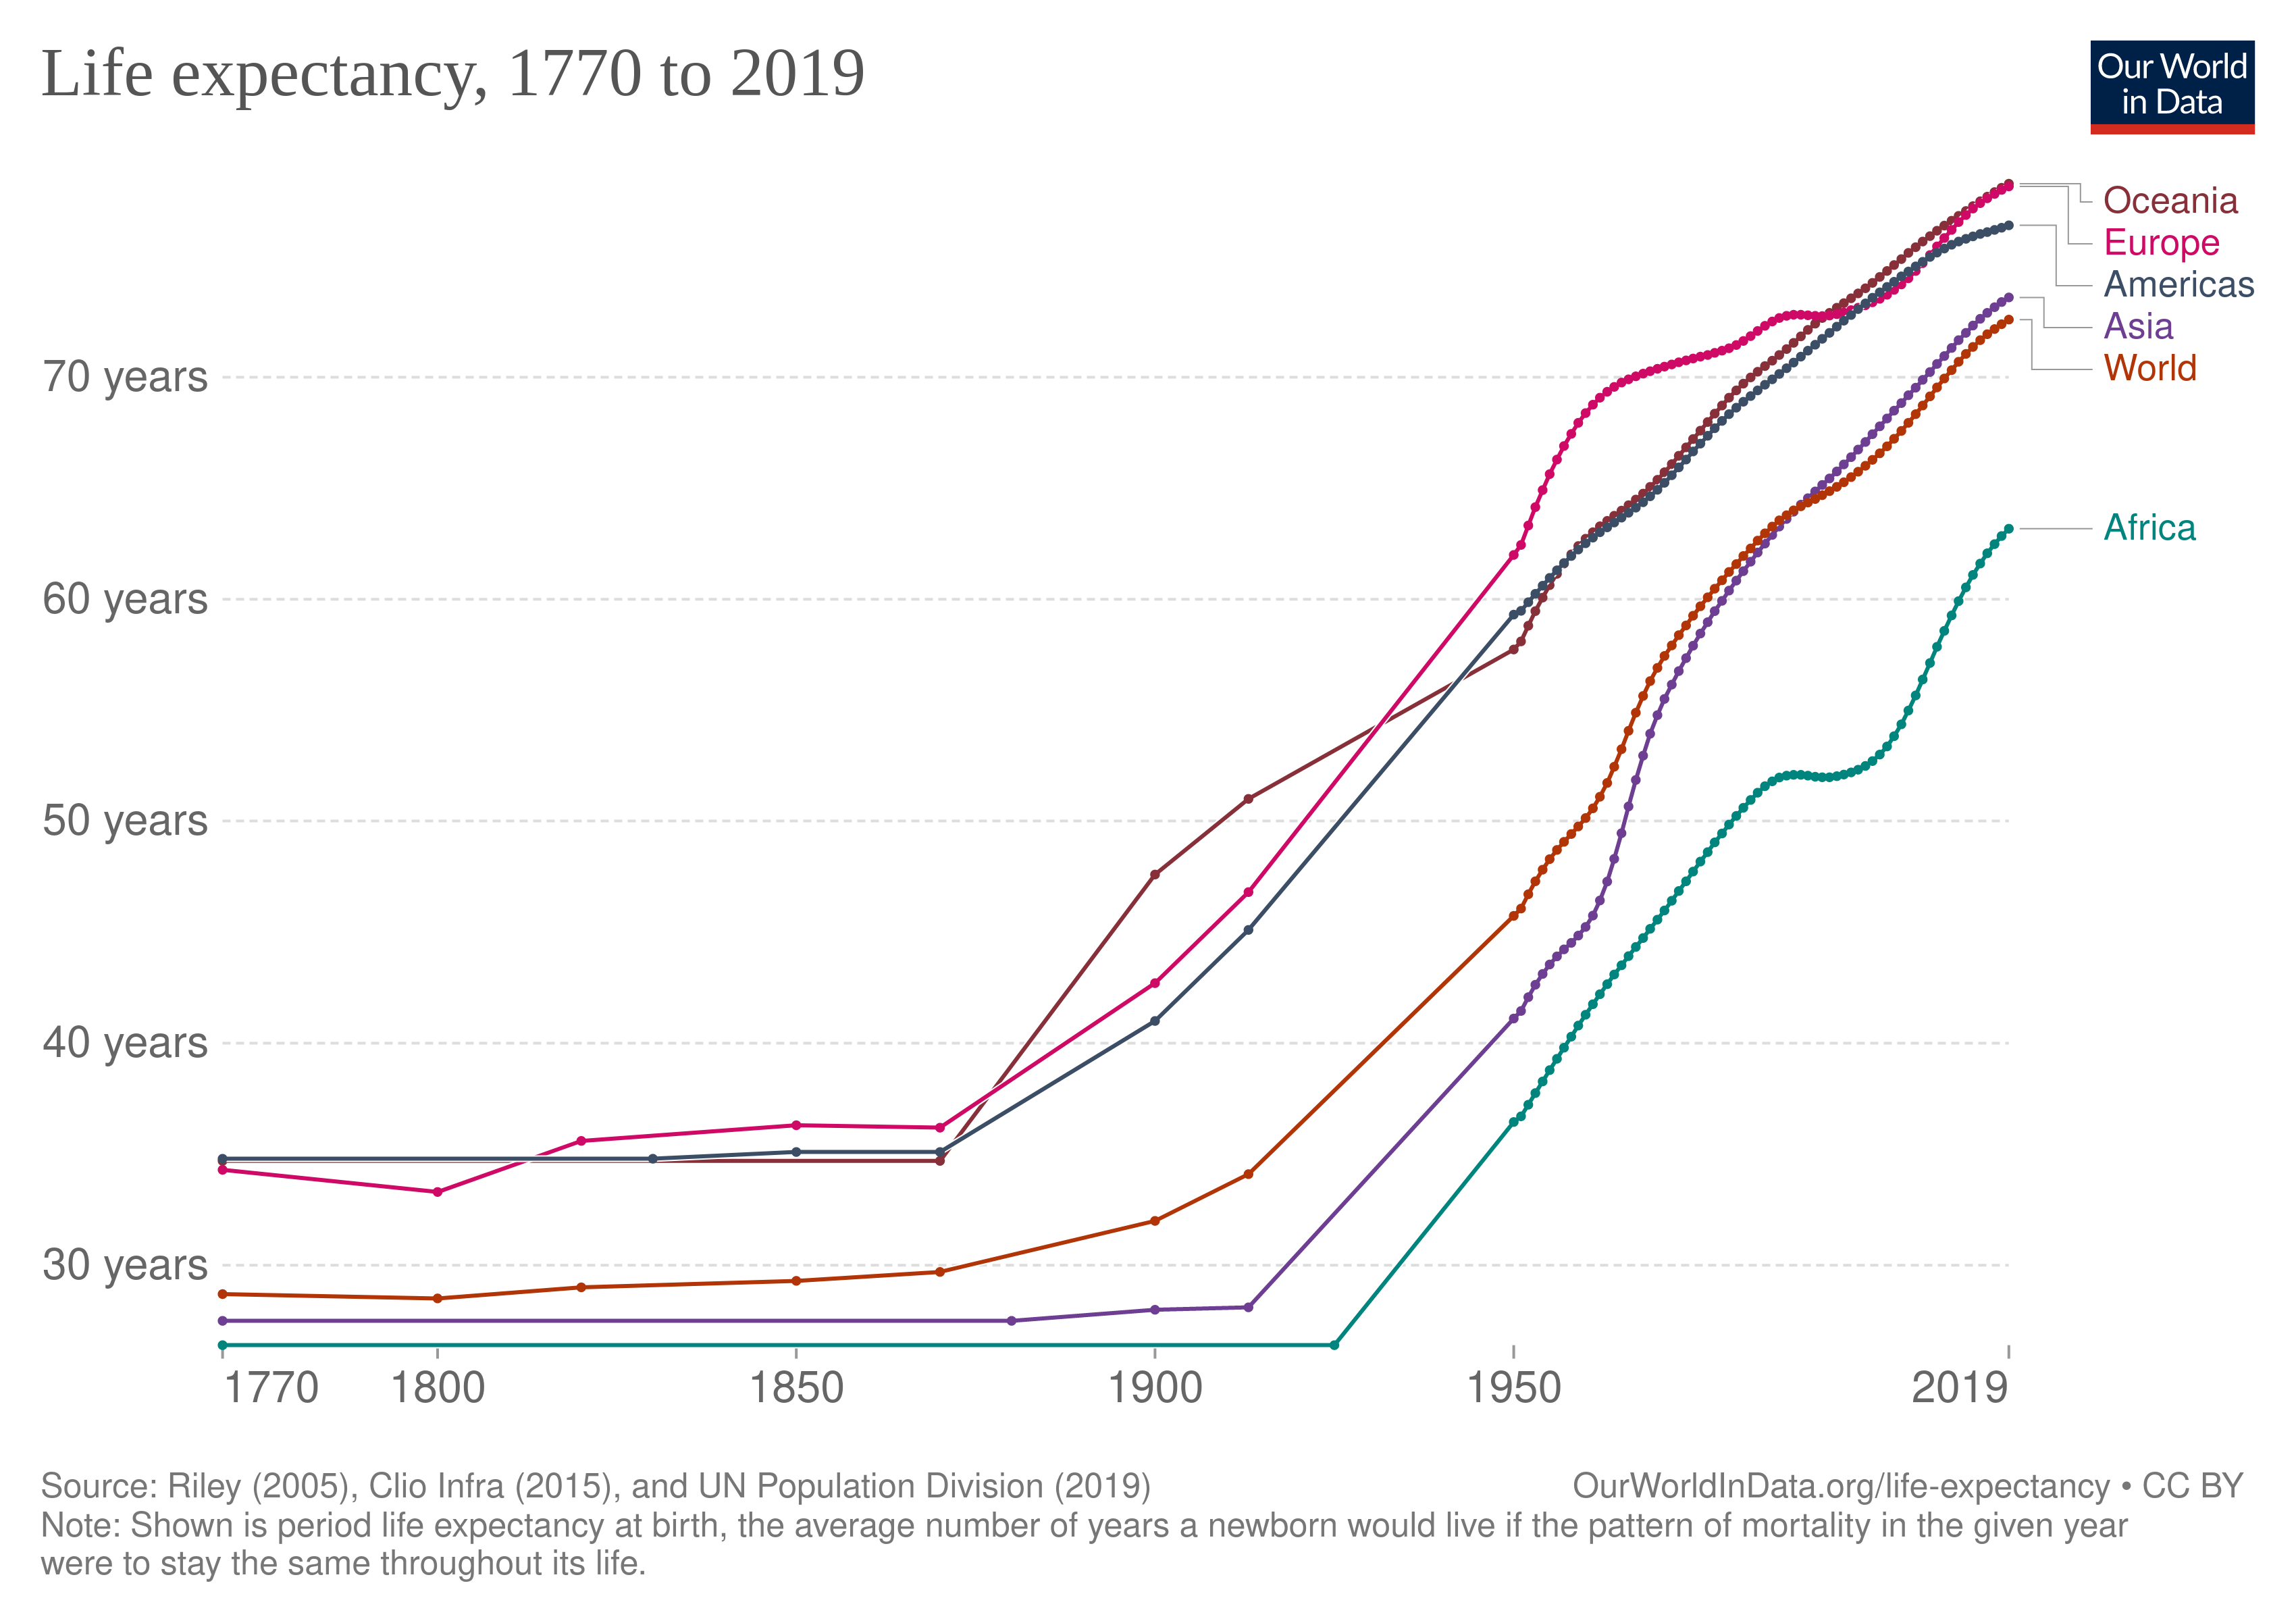
\includegraphics[width=12cm]{figures/life-expectancy}
  \caption {Очаквана продължителност на живота за различни региони през периода 1770-2019 \cite{zijdeman2016}.}
  \label{fig:life_expectancy}
\end{figure}

\paragraph{}
Застаряването на населението би оказало неблагоприятен ефект и върху икономиката на държавите. Първо, заради увеличаването на дяла на хора, които не участват в работната сила. Второ, поради това, че здравните системи ще бъдат допълнително натоварени с по-голям брой хора в напреднала възраст, за които рисковете от хронични заболявания са значително по-големи.


\section[Молекулярно-биологични теории за стареенето]{Молекулярно-биологични теории\\ за стареенето}
\subsection{Общи молекулярно-биологични процеси}
\paragraph{}
В тази секция ще разгледаме фунадменталните принципи на генетиката. Ще направим кратък обзор на начина на съхранение на генетичната информация и процесите, чрез които тя бива изразена, за да повлияе на фенотипа. С това целим да дадем базов биологически контекст, чрез който да бъдат разбрани по-нататъшните разработки и биоинформатични анализи.

\paragraph{}
Дезоксирибонуклеиновата киселина (ДНК) представлява две вериги от спираловидно преплетени полимери, които съдържат генетичната информация при всички клетъчни форми на живот. Полимерите са създадени от последователности от мономери - нуклеотидни бази. В ДНК се изпозлват четири вида бази - аденин (А), цитозин (C), гуанин (G) и тимин (T). Базите A и T образуват двойки помежду си, както и базите C и G. Казваме, че двете нишки на ДНК са комплиментарни. Всеки ген може да бъде разположен на коя да е от двете нишки на ДНК и е описан от дълга последователност от нуклеотидни бази \cite[стр. 301-310]{klug2014}.

\paragraph{}
Най-често крайната цел на един ген е кодирането на протеин. Първата стъпка към това е транскрипцията, при която ензимът ДНК-полимераза копира информацията от ДНК в комплиментарна РНК молекула \cite{sims2004}. При РНК, базата T е заменена с урацил (U). Първичната РНК молекула (pre-mRNA) преминава прецес на сплайсване, при който части от нея (интрони) биват изрязвани и остранени. Останалите части (екзони) се свързват отново. Така се образува зрялата mRNA, която бива транслирана в рибозомите, като на всеки кодон (група от три нуклеотидни бази) се съпоставя определена амино-киселина (виж фиг. \ref{fig:transcription_splicing_translation}). Верига от амино-киселини образува протеин \cite[стр. 412-420]{klug2014}.

\begin{figure}[h]
  \centering
  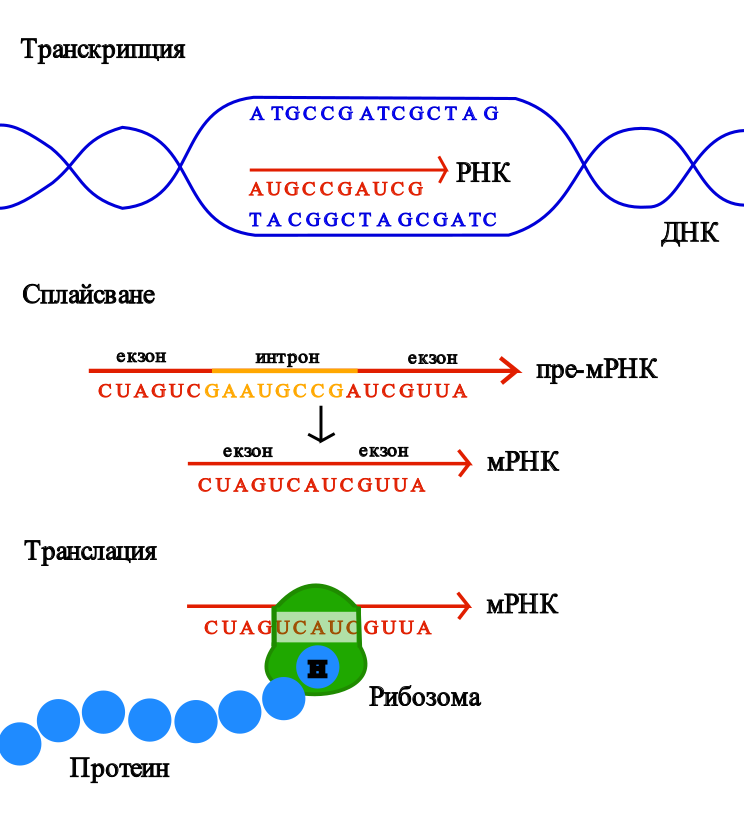
\includegraphics[width=12cm]{figures/transcription_splicing_translation}
  \caption {Графична репрезентация на процесите на транскрипция, сплайсване и транслация}
  \label{fig:transcription_splicing_translation}
\end{figure}

\subsection{Теории за стареенето}
\paragraph{}
Стареенето е въпрос, който вълнува учените от дълго време. През 1990-та, Медведев твърди, че вече съществуват над 300 теории за стареенето \cite{medvedev1990}. Въпреки постигнатият значителен прогрес през последните години в областта на геронтологията, причините за стареенето все още оставан ненапълно обяснени. Това се дължи на факта, че стареенето е сложен процес, в който са намесени множество фактори. Все още липсва голяма обединяваща теория на стареенето, която да обясни изцяло процеса, но съществуват множество теории, които дават добра представа за различни негови аспекти \cite{vina2007}. Следва кратък преглед на основните теории:

\subsubsection{Натрупване на геномни изменения}
\paragraph{}
Изменения в ДНК молекулите могат да настъпят както в следствие на вътрешноклетъчни фактори, така и поради въздействието на външни мутагени. Примери за вътрешноклетъчни фактори са случайни грешки при репликация и оксидативния стрес, предизвикан от натрупването на свободни радикали \cite{wang1998}. Външните мутагени могат да бъдат разделени на три вида - физични, химични и биологични. Пример за физичен мутаген е радиацията \cite{breimer1988}, a за биологичен вирусните инфекции, които също могат да предизвикат генетични мутации. Измененията в ДНК молекулите включват различни видове мутации като точкови мутации, делеции и инсерции, транслокации, инверсии и др.\\\\
Съществуват механизми, чрез които клетките засичат мутациите и ги поправят. Основни такива механизми са гените ATM и TP53. Все пак, тези механизми не са ефективни на 100\% и ефективността им допълнително спада с възрастта \cite{auley2017}. В резултат, в течение на времето, ДНК молекулите акумулират все повече мутации. Смята се, че тази геномна нестабилност е един от основните фактори, допринасящи за процеса на стареенето \cite{vijg2013}.

\subsubsection{Скъсяване на теломерите}
\paragraph{}
Теломерите са регион, намиращ се в края на хромозомите, в който се съдържат повтарящи се поредици от нуклеотидни бази. Те служат за предпазване на хромозомата от рекомбинация и постепенна деградация и дават възможност на клетката да различава края на хромозомата от случайни прекъсвания, при които биха били активирани механизмите за поправка на ДНК \cite{griffith1999}. При всеки цикъл на делене на клетката, теломерите се скъсяват поради непълното синтезиране на изоставащата нишка от ДНК полимеразата \cite{koliada2015}. Този проблем се компенсира донякъде от ензима теломераза, който пренася своя собствена РНК молекула и я използва като шаблон, спрямо който да удължи скъсения теломер. Въпреки това, недостатъчната експресия на теломеразата води до постепенното скъсяване на теломерите. Това може да доведе до загуба на репликативна способност на клетката и блокирането на клетъчния ѝ цикъл, процес известен като клетъчно стареене \cite{muraki2012}. Установено е, че първоначалната дължина на теломерите няма връзка със стареенето при различни видове, но скоростта на тяхното скъсяване има значителна корелация със продължителността на живота им \cite{whittemore2019}.

\subsubsection{Клетъчно стареене}
TODO

\subsubsection{Епигенетични изменения}
TODO

\section[Генетични фактори, влияещи на процеса на стареене]{Генетични фактори, влияещи на процеса\\ на стареене}
\paragraph{}
В секция 2.2.2 беше представен кратък обзор на различните биологични процеси, които способстват процеса на стареене. Уместен е въпросът дали има определени генетични фактори, които оказват въздействие на тези процеси. Ако това е така, бихме могли да очакваме, че съществуват генни алели, които забързват или забавят стареенето. В текущата глава ще разгледаме въпроса за съществуването на такива генни алели, както и за начините им на действие и методите за изследването им. 

\subsection[Видове генетични мутации, влияещи на стареенето]{Видове генетични мутации, влияещи\\ на стареенето}
\paragraph{}
Два от биологичните процеси, разгледани в секция 2.2, за които се смята, че причиняват стареенето, са натрупването на геномни мутации и клетъчното стареене. Един протеин, който играе важна роля и в двата процеса е p53. Той се кодира от хомолози на един и същи ген в различни организми. При хората това е генът TP53. Протеинът p53 има роля за предотвратяването на натрупване на геномни мутации и спирането на туморогенезиса. Той бива активиран в отговор на увреждания на ДНК, експресия на онкогени и дисфункция на рибозомите. Функциите на p53 включват активиране на гени, свързани с поправката на ДНК, спиране на клетъчния цикъл, за да се предотврати размножаване на клетката, докато има уреждания в ДНК, активиране на клетъчното остаряване и инициране на апоптоза (клетъчна смърт) \cite{toufektchan2018}. В изследвания на хора е установено, че полиморфизми в TP53 могат да доведат до удължаване на живота, но да увеличат и смъртността от рак \cite{heemst2005}. Това демонстрира и крехкия баланс между ползи и вреди, които дадени алели могат да носят.

\paragraph{}
Протеинът Telomeric repeat-binding factor 1, кодиран от генът TERF1 при хората, е основен компонент от shelterin комплекса, който има важна роля в защитата и репликацията на теломерите. Изследвания показват, че увеличаването на експресията на TRF1 в зрели мишки (на 1 година) и възрастни мишки (на 2 години), посредством генна терапия, може да забави настъпването на патологии, свързани със стареенето \cite{derevyanko2017}.

\paragraph{}
TODO: пример свързан с епигенетични процеси

\paragraph{}
Тези примери не са изолирани изключения. В научната литература могат да бъдат намерени много гени, за които изследвания са открили асоциация със стареенето. Публичната база данни Human Ageing Genomic Resources (HAGR), представлява колекция от ресурси за изследването на стареенето при хората. Някои записи в HAGR са включени на база установена директна връзка между даден ген и стареенето, докато други са включени на база ролята им в различни човешки патологии. Много от записите са подбрани, тъй като за техни хомолози в други организми е била открита връзка със стареенето. HAGR предоставя и набор от софтуерни инструменти (предимно Perl и SPSS скриптове) за различни видове биоинформатичен анализ. Към момента в HAGR са налични над 300 човешки гена, за които се предполага, че имат потенциална връзка със стареенето \cite{tacutu2018}.
 
\section[Обзор на съществуващи биоинформатични решения]{Обзор на съществуващи\\ биоинформатични решения}
\subsection{VCF файлове}
\paragraph{}
Variant Call Format (VCF) е стандартен файлов формат, който се използва за описване на генетичните полиморфизми за дадена секвенция (за примерен файл виж фиг. \ref{fig:example_vcf}). VCF е текстов файлов формат с разделители-табулации (tab-delimited), който често бива съхраняван в компресиран вид, с цел оптимизиране на хардурерните ресурси, като дори компресиран може да бъде индексиран за бързо търсене. Във VCF могат да бъдат описани различни видове полиморфизми, от прости като точкови мутации, инсерции и делеции до по-сложни като например инверсии. VCF може да съдържа коментари, заглавен ред и редове за данни. В редовете за данни, всеки ред показва един полиморфизъм, като обикновено се използват стандартни референтни геноми, спрямо които се определят полиморфизмите. Файловият формат позволява и добавянето на богата анотация и потребителски-дефинирани полета. VCF стандартът е разработен за 1000 Genomes Project, а впоследствие е добил широка приемственост в биоинформатичната общност \cite{danecek2011}.

\begin{figure}[h]
  \centering
  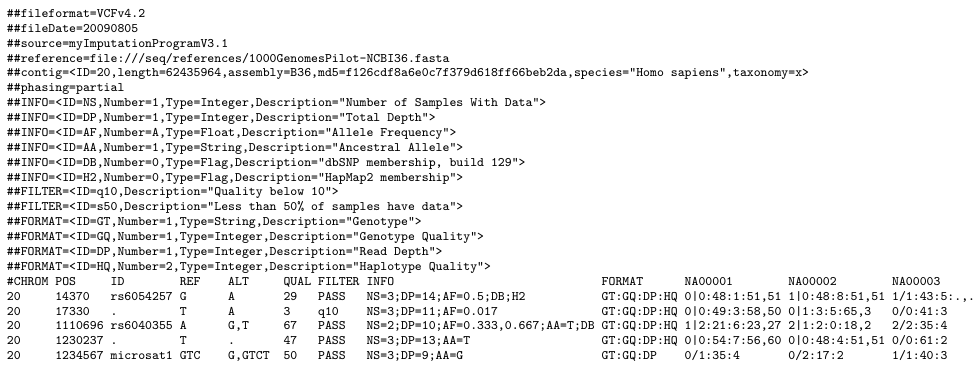
\includegraphics[width=17cm]{figures/vcf}
  \caption {Примерен VCF файл}
  \label{fig:example_vcf}
\end{figure}


\subsection{Анотация на генетични варианти}
\paragraph{}
С напредъка на технологиите за секвениране способността за бързо генериране на големи обеми от данни за генетични варианти бързо расте. Същевременно се образува все по-голяма пропаст между възможностите за генериране на нови сурови данни и възможностите за извличане на полезна информация и познание от тях \cite{yang2015}. Основна стъпка за разбирането на суровите данни с генетични варианти е анотирането им. Анотацията представлява процес, при който към генетичните варианти се добавя допълнителна функционална информация \cite{mccarthy2014}. Това може да бъде информация към кои кодиращи секвенции и гени се отнася варианта, оценка на степента му на въздействие, индикация дали се променят аминокиселините на кодирания протеин \cite{cingolani2012}, предсказване на структурните и функционални промени в протеина \cite{mccarthy2014} и др.
\subsubsection{snpEff}
\paragraph{}
SnpEff е софтуер с отворен код, който може бързо да анотира и категоризира генни варианти на база на ефекта, който те биха имали върху анотираните гени. SnpEff поддържа анотацияа на различни видове полиморфизми, като например единични нуклеотидни полиморфизми (SNPs), множествени нуклеотидни полиморфизми (MNPs) и вмъквания-изтривания (Indels) \cite{cingolani2012}. SnpEff разполага с много богата база данни от различни референтни геноми, с които може да работи, а дава възможност на потребителя да използва и свой собствен референтен геном. Основният формат, с който SnpEff работи е VCF. След обработката на входния VCF файл, съдържащ по един полиморфизъм на ред, SnpEff добавя една или повече анотации за всеки полиморфизъм в полето INFO, като всяка анотация има ключ „ANN“. Някои от по-важните анотации, които SnpEff предоставя са: идентификация на генът, с който е свързан полиморфизма; идентификатори на транскриптите, които полиморфмизмът засяга; оценка на ефекта на полиморфизма и на промените, които би причинил в аминокиселинния състав на протеина, който кодира. SnpEff е имплементиран на програмния език Java, което го прави лесно преносим и му дава възможност да работи на изключително голям набор от операционни системи и устройства \cite[стр. 9-10]{schildt2020complete}.
\subsubsection{VEP}
\paragraph{}
\subsubsection{Annovar}
\subsection[Филтриране и анализ на генетични варианти]{Филтриране и анализ на генетични\\ варианти}
\subsubsection{snpSift}
\paragraph{}
SnpSift е софтуер за филтриране и промяна на VCF файлове, съдържащи анотирани генетични варианти. Чрез SnpSift могат да се извършат различни операции, като например филтриране по геномен регион, разделяне на файла по хромозома, извличане на определени полета, допълнително анотиране спрямо външни бази данни, както и филтриране с потребителски дефиниран логически израз. Филтрирането с потребителски израз работи посредством рекурсивна граматика, която може да обработва изрази с произволна сложност \cite{cingolani2012sift}. Това прави snpSift доста мощен инструмент за лесна обработка и анализ на генетични варианти и извличане на информация от тях. SnpSift, също като SnpEff, е имплементиран на програмния език Java, което му дава голяма преносимост върху различни операционни системи и платформи \cite[стр. 9-10]{schildt2020complete}.
\subsubsection{??? TODO}
\subsection{Геномни браузъри}
\subsubsection{UCSC Genome Browser}
\subsubsection{IGV Genome Browser}
\subsection{Нагъване на протеини}
\subsubsection{Подходи}
\subsubsection{AlphaFold}
\subsection{Интегрирани софтуерни решения}
\subsubsection{Galaxy Project}
\chapter{Цели и задачи}
\section{Цели на дипломната работа}
Дипломната работа има за цел създаването интегрирана софтуерна система за биоинформатичен анализ на геномни варианти, която има следните характеристики:
\begin{itemize}
  \item Да приема входни данни за генетични варианти посредством стандартен VCF файлов формат.
  \item Да може да анализира генетични варианти и да предоставя подробен доклад, съдържащ:
  	\begin{itemize}
  		\item Идентификация на гените, засегнати от полиморфизмите.
  		\item Асоцииране на тези гени с процеса на стареенето.
  		\item Оценка на тежестта на откритите варианти.
  		\item Предсказване на откритите варианти върху процеса на транслация и протеиновата структура.
  		\item Предсказване и визуализация на на триизмерните протеинови (третични) структури.
 	\end{itemize}
  \item Да разполага с уеб-базиран потребителски интерфейс, за улеснено ползване от
потребители, които не са компютърни специалисти.
  \item Да разполага с потребителски интерфейс, работещ в командния ред на операционната система, позволяващ
интеграцията на софтуера в други биоинформатични системи.
\end{itemize}
\section{Задачи}
За постигане на целите, описани в предишната секция се предвижда следния списък от задачи:
\begin{enumerate}
	\item Интегриране на софтуер за анотация на генетични варианти към програмното решение.
	\item Филтрация на анотираният VCF с генетични варианти, така че да съдържа единствено полиморфизми, засягащи гени, които потребителят е решил да изследва.
	\item Анализ на наличните данни и моделиране на релационна база данни, в която данни да бъдат съхранявани с цел последващо изпълняване на разнообразни аналитични заявки.
	\item Разработване на уеб-базиран потребителски интерфейс, който да включва:
		\begin{enumerate}
			\item Възможност за създаване и управление на генетични множества, спрямо които да бъдат изследвани входните VCF файлове с генетични варианти.
			\item Възможност за качване на входен VCF файл, съдържащ генетични варианти.
			\item Набор от страници за изследване на резултатите за обработен VCF файл.
		\end{enumerate}
	\item Намиране на модифицираната полипептидната поредица на модифицираните от генетичен вариант протеини.
	\item Интегриране на софтуер за предсказване на третичната (триизмерна) структура на протеини към програмното решение.
	\item Интегриране на решение за визуализация на биолгоични макромолекули, с цел представяне на триизмерната третична структура на референтния и модифицирания протеин с цел сравнението им.
\end{enumerate}
\chapter[Използвани софтуерни решения]{Използвани софтуерни\\ решения}
\section{Flask}
\paragraph{}
Flask \cite{flask} е минималистичен framework (преизползваема платформа, която подпомага разработването на софтуер) за създаване на уеб приложения с програмния език Python. Класифицира се като минималистичен, тъй като не налага използването на определени библиотеки и инструменти, а оставя избора да бъде направен от програмиста. За разлика от много други уеб framework решения, Flask не включва определени компоненти и библиотеки за стандартни нужди като връзка с бази данни, валидация на потребителски входни данни, автентикация и др. Вместо това, предоставя възможности за разширяване, към които могат да се вградят произволни външни библиотеки и компоненти.

\paragraph{}
Flask (v2.1.2) е основен компонент в програмното решение, като го използваме за изграждането на уеб-базирания потребителски интерфейс. Flask се грижи за обработката на HTTP заявките, насочването им към правилния контролер-метод, изграждането на статичните страници (чрез шаблонни страници, рендерирани от библиотеката Jinja), поддържането на потребителската сесия и др.
\section{DuckDB}\label{sec:duckdb}
\paragraph{}
DuckDB \cite{raasveldt2019} е система за управление на бази данни, която позволява изпълняването на SQL заявки, докато е вградена в друг процес. Това означава, че базата данни не се нуждае от отделен сървър, който да управлява базата данни и да изпълнява заявките. Вместо това, системата може да бъде вградена в програма под формата на библиотека с функции, позволяващи работа с базата данни, която представлява отделен файл на файловата система. В този аспект, DuckDB прилича на популярната база данни SQLite \cite{sqlite2020hipp}. DuckDB е предвидена за изпълняването на аналитични заявки, известни още като OLAP (Online Analytical Processing). При този тип заявки, най-често се използва сравнително малко подмножество от наличните колони, но за сметка на това се прави обработка на всички налични редове. За да се осгури добра производителност за този тип употреба, DuckDB използва техниката за векторизация на заявките, при която множество стойности биват изчитани и обработвани накуп, вместо една по една, като по този начин се амортизира сложността на итерацията \cite{kersten2018}.

\paragraph{}
За нашето решение, избрахме да използваме DuckDB (v0.4.0), защото основните заявки, които се изпълняват са аналитични по своята природа и обработват голямо количество от редове. Заявките за писане, и особено транзакционните такива, са редки. В допълнение, липсата на отделен сървър за базата данни улеснява инсталацията на софтуера за потенциалните му потребители.
\section{Pandas}
\paragraph{}
Pandas \cite{reback2020pandas} е популярна библиотека за програмния език Python за анализ и манипулация на данни, създадена през 2008 година. Pandas предоставя DataFrame стуктура от данни, представляваща колекция от данни, представени в табличен вид. Pandas включва богат набор от функции за операции като анализ, трансформация, групиране, агрегация, преоразмероване, сливане и разделяне, четене/писане от и към различни видове файлови формати и др. Основните критични пътища са имплементирани на C и CPython, значително оптимизирайки производителността.

\paragraph{}
Повечето от операциите в програмното решение засягат обработката на голям обем от данни от структурирани данни, което прави използването на Pandas удачно. Също така, DuckDB предоставя интерфейс за извличане на резултати от заявки и за подаване на данни, при който се използват Pandas DataFrame обекти. Разработчиците на DuckDB препоръчват използването на тези интерфейси, когато обемът на данните е по-голям, поради по-голямата им ефективност. Използвана е версия 1.4.2.
\section{PyVCF3}
\paragraph{}
PyVCF3 \cite{pyvcf3} е наследник на библиотеката PyVCF, адаптирано за съвместимост с версия 3 на програмния език Python. PyVCF е библиотека за синтактичен анализ на VCF файлове, която позволява прочичтането на VCF файлове и зареждането им в Python класове и структури от данни. PyVCF се опитва да обработи „\#\#INFO“ и „\#\#FORMAT“ редовете, за да отгатне структурата на данните във входния файл. Ако това не е успешно, се обръща към дефинициите в VCF стандарта.

\paragraph{}
Програмното решение използва PyVCF3 (v1.0.3) за да прочете входните или междинните VCF файлове. Веднага след прочитането, данните се зареждат в Pandas DataFrame, чрез който биват обработвани.

\section{Samtools и Tabix}\label{sec:samtools_tabix}
\paragraph{}
Форматът SAM (Sequence Alignment/Map) е стандартен формат за съхраняване на голям брой подравнявания на нуклеотидни последователности. BAM е бинарен файл, представляващ компресирана версия на съответния му SAM файл. Samtools \cite{li2009} софтуер за обработка на SAM и BAM файлове, включващ редица операции като сортиране, инспектиране, обединяване на файлове и др.

\paragraph{}
Tabix е 	програма за индексиране на делимитирани с табулация файлове, съдържащи геномни позиции. След индексирането на файл, Tabix позволява бързото намиране на редове, съдържащи информация за конкретни геномни региони. Важно необходимо условие за използването на Tabix за индексиране на файл е файлът да бъде сортиран предварително спрямо геномната позиция. 

\section{Pysam}\label{sec:pysam}
\paragraph{}
Pysam \cite{pysam} е библиотека за Python, която позволява четенето и манипулирането на файлове в SAM и BAM формат. Pysam представлява тънка обвивка около samtools и tabix и позволява лесното взаимодействие с тези инструменти от Python програми.

\paragraph{}
В програмното решение, Pysam (v0.19.1) се използва за компресиране и индексиране на междинните VCF файлове, които програмата извлича след анотирането и филтрирането на входния VCF.

\section{HGVS}\label{sec:hgvs}
\paragraph{}
Human Genome Variation Society (HGVS) е организация, занимаваща се с генетични варианти при хората, дала името и на стандартна номенклатура за описване на варианти на ДНК, РНК, протеини и други свързани с генетиката макромолекули. HGVS стандарът е широкоприет \cite{dunnen2016}. Общият формат за описване на вариант е „референция:описание“. Например, „NM\_004006.2:c.4375C>T“ описва вариант на транскрипта NM\_004006.2, при който в кодиращото ДНК цитозина от позиция 4375 е подменен от тимин.

\paragraph{}
Hgvs \cite{wang2018} е също така и името на библиотека за Python за манипулирането на варианти на поредици, използвайки HGVS номенклатурата. Hgvs позволява синтактичен анализ, форматиране, валидация и нормализиране на варианти на поредици от ниво геном, транскриптом или протеом.

\paragraph{}
В програмното решение се използва версия 1.5.2 на пакета за да се направи синтактичен анализ на HGVS номенклатурата, получена при анотацията посредством SnpEff, и да се изведе модифицирания протеин.

\section{Bulma}
\paragraph{}
Bulma е CSS framework, който предоставя готови компоненти и функционалности за стилизиране на уеб страници и разработване на потребителски интерфейси. Bulma се съдържа изцяло в един единствен CSS файл, който предоставя богата колекция от класове за стилизране на HTML. Bulma предоставя и множество стандартни компоненти за изграждане на потребителски интерфейси като: менюта, контейнери за съобщения, навиганционни ленти, модални прозорци, страниране, етикети и др. В програмното решение е използвана версия 0.9.4 на Bulma.

\section{IGV}
\paragraph{}
IGV (Integrative Genomics Viewer) е инструмент за визуализация и интерактивно изследване на разнообразни, големи по обем геномни колекции от данни . Посредством IGV могат гъвкаво да се интегрират широк спектър от различни типове геномни данни, като например подравнени поредици, мутации, експресия на гени, метилация, геномни анотации и др. IGV позволява на потребителя да изследва данните си на различни нива на резолюция, като дава възможност за приближаване и отдалечаване в реално време \cite{robinson2011}\cite{robinson2017}. Данните могат да бъдат зареждани както от публични онлайн бази данни, така и локално от данните, с които разполага потребителя.

\begin{figure}[h]
  \centering
  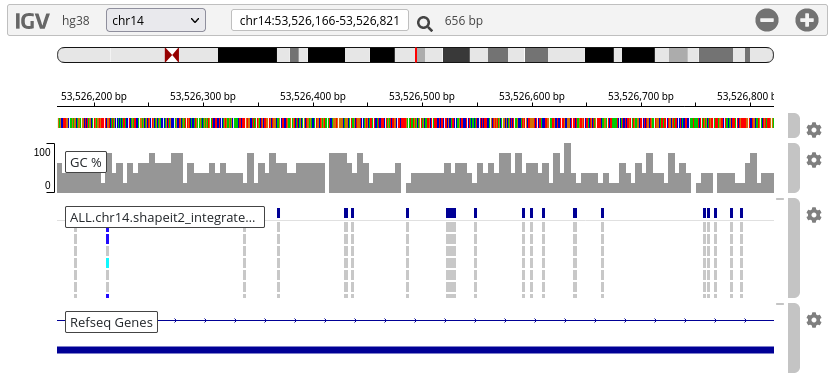
\includegraphics[width=17cm]{figures/igv_example}
  \caption {Примерна визуализация с IGV}
  \label{fig:ign_example}
\end{figure}

\paragraph{}
В програмното решение, IGV е интегриран в страницата за изследване на вариантите за определен ген.

\section{Външни генетични библиотеки}

\subsection{HGNC}\label{sec:hgnc}
\paragraph{}
HGNC (HUGO Gene Name Nomenclature Committee) е организация отговорна за одобрението на уникални символи и имена за човешки гени, протеини, некодиращи РНК гени и псевдогени, с цел улесняване на комуникацията между учените \cite{povey2001hugo}. HGNC също предоставят публична база данни с пълната, одобрена от организацията, номенклатура. Тя е достъпна на адрес „genenames.org“ и също така предоставя REST API, чрез който информацията може да бъде достъпвана програматично. Освен номенклатурата, базата данни предоставя и идентификатори за артефакта на различни често използвани външни бази данни, като например Ensembl и UniProt.

\paragraph{}
Програмното решение използва REST API услугата на HGNC за да извлича името и обща информация за гени, включително идентификатори от други бази данни. Тези идентификатори се използват за генериране на линкове към, с които потребителя да може да изследва въпросният ген в по-голяма дълбочина.

\subsection{Ensembl}\label{sec:ensembl}
\paragraph{}
Ensembl е система за генериране и дистрибуция на геномна анотация, като например гени, генни варианти, генетична регулация и сравнителна геномика за множество видове сред гръбначните организми и други моделни организми. Ensembl интегрира експериментални и референтни данни от множество източници на едно място. Към 2020 година, Ensembl съдържа анотираните геноми на 227 различни вида \cite{yates2020}. Информацията, предоставяна от Ensembl, също така може да бъде извличана програматично чрез REST API.

\paragraph{}
Програмното решение използва REST API услугите, предоставяни от Ensembl, за да извлича референтната аминокиселинна поредица на протеините, които потребителя изследва.

\subsection{NextProt}\label{sec:nextprot}
\paragraph{}
NextProt е платформа, която се стреми да дава цялостна и богата информация за човешките протеини. Разработва се от Швейцарския Институт по Биоинформатика. Използва както информация от експертно-модерираната база данни UniProtKB/Swiss-Prot, така и внимателно селектирана информация от експерименти с високопроизводително секвениране \cite{lane2011}. NextProt съдържа богата информация за функцията на протеините, биологичните пътища, в които те участват, както и молекулярните процеси, с които са свързани.

\paragraph{}
Програмното решение използва REST API услугата на NextProt за да извлича функциите, молекулярните процеси и биологичните пътища, с които се свързва даден протеин. Информацията се предоставя на потребителя, за да даде контекст за значението на протеина, който бива изследван.

\chapter{Резултати}
\paragraph{}
Въпреки огромното значение на процеса на стареене за индивида и обществото като цяло, науката все още не може да го обясни напълно, нито да намери достатъчно ефективни решения за справяне с негативните ефекти, които той предизвиква. Откритите асоциации между определени генетични варианти и стареенето означава, че бъдещите изследвания трябва да включват и изследване на генетични полиморфизми. Този тип изследвания генерират големи обеми от данни, но съществуващият биоинформатичен софтуер за целта изисква високо ниво на подготовка в областта на информационните технологии. Биолозите и генетиците, които искат да разберат данните, получени от геномните секвенирания, често трябва да изграждат сложни системи от различни програми. Свързването им често включва писането на програмни скриптове.

\paragraph{}
С цел да облекчим работата при бъдещи изследвания на генетични полиморфизми, свързани със стареенето, и да направим такива изследвания по-достъпни, разработихме интегрирана биоинформатична система, която позволява анализирането и интерпретирането на данни за генетични варианти посредством удобен, уеб-базиран, графичен интерфейс. Софтуерът ни е имплементиран на програмния език Python и е достъпен за свободно ползване без ограничения, като кодът му е отворен и достъпен на адрес \url{github.com/mzdravkov/gene_variants}. Софтуерът има за цел да бъде лесен за инсталиране и използване.

\paragraph{}
В процеса на разработка установихме, че същите принципи, които прилагаме за изследване на полиморфизми, свързани със стареенето, могат да бъдат приложени и върху други видове изследвания, като това изискваше съвсем малка генерализация на предвиденото софтуерно решение. В резултат, разработихме възможност за управление на различни множества от гени, като при подаване на VCF файл с генетични варианти, потребителят може да избере кое генно множество да бъде анализирано при обработката на полиморфизмите.

\section{Софтуерна архитектура}
\paragraph{}
Софтуерната архитектура на системата може да се раздели на четири слоя. Интерфейсен, включващ командния ред и уеб интерфейса с неговите страници, стилове и JavaScript код, който се изпълнява от браузъра на потребителя. Вторият слой включва контролерите, които обработват HTTP заявките, изпращани от уеб интерфейса. Третият слой се занимава с обработката или извличането на данни. В него се включват модулът за обработка на входни VCF файлове, модулите за извличане и анализ на данни от базата данни и модулът за извличане на данни от външни, онлайн бази данни (фиг. \ref{fig:software_architecture}).

\begin{figure}[h]
  \centering
  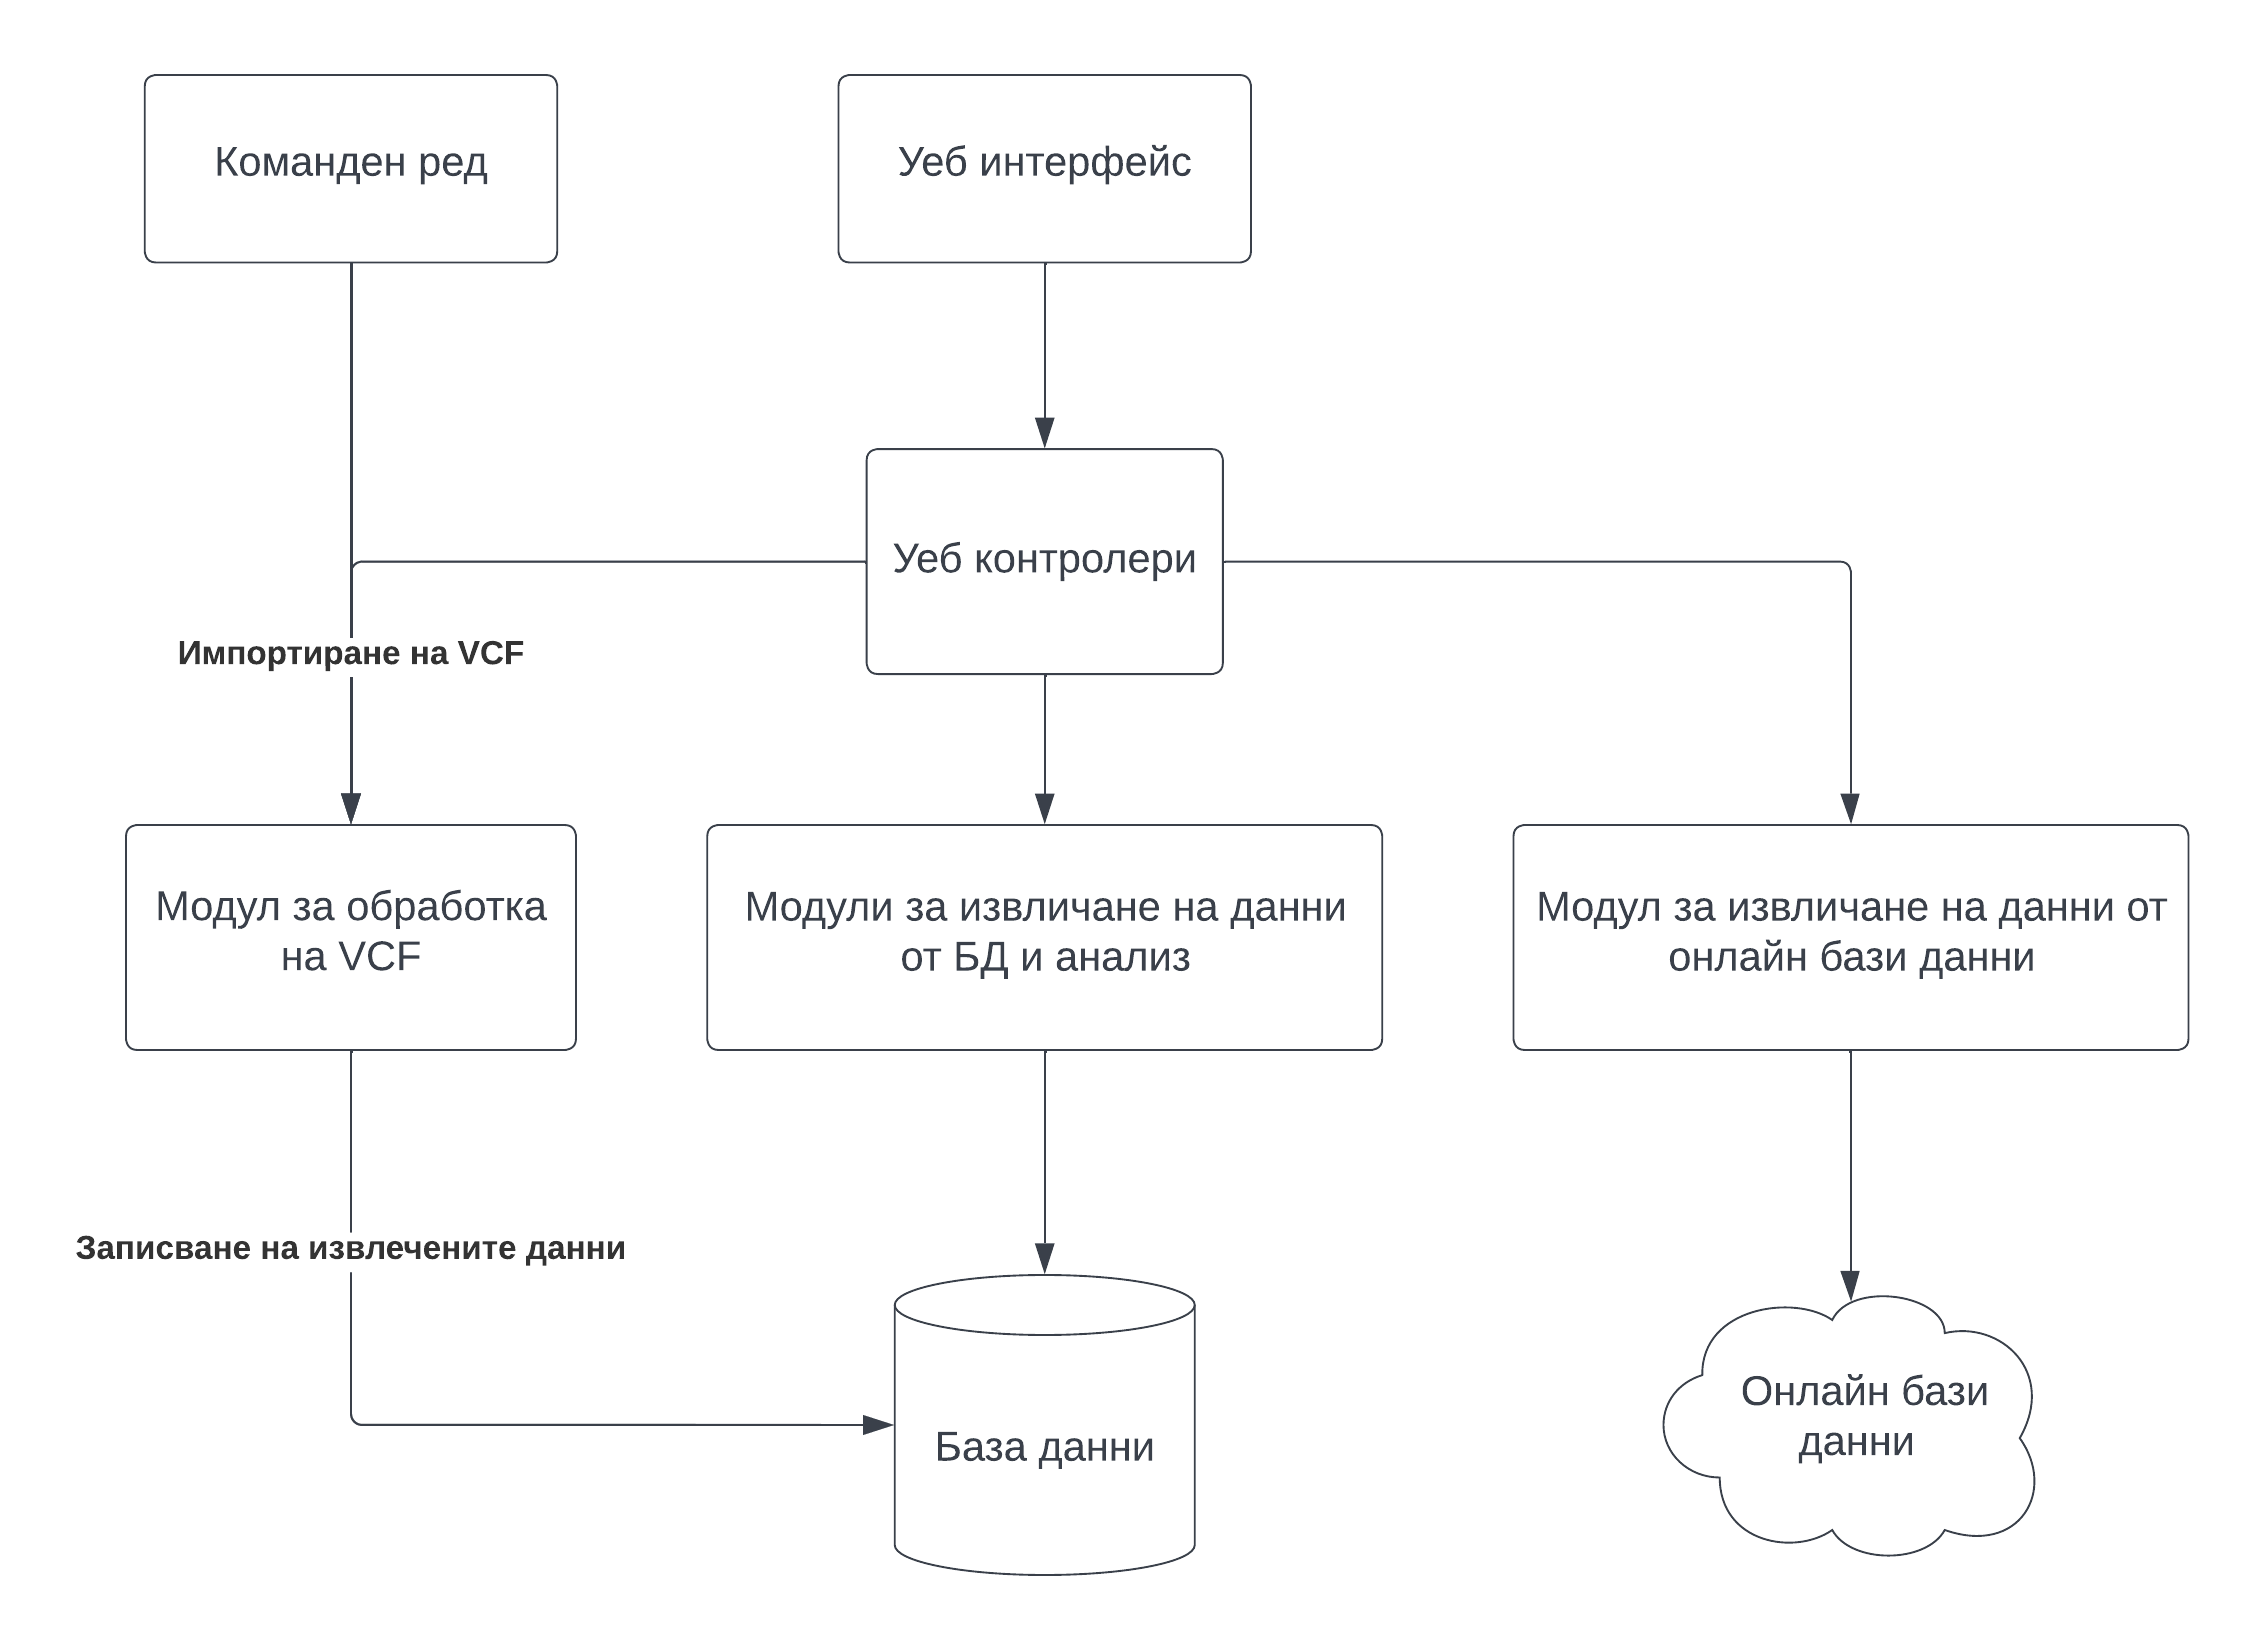
\includegraphics[width=17cm]{figures/software_architecture}
  \caption {Диаграма на софтуерната архитектура на разработеното решение}
  \label{fig:software_architecture}
\end{figure}

\section{База данни}
При изборът на тип на базата данни се спряхме на релационна база данни. Причините за това са няколко. Първата съществена причина е това, че структурата на данните е предварително ясна и промени по нея са малко вероятни. Това е така, тъй като структурата е базирана на информацията налична във VCF файловете и тази, предоставяна от софтуера за анотация (SnpEff). VCF форматът е дефиниран в общоприет стандарт \cite{danecek2011variant}, който не се променя често. Анотациите, предоставяни от SnpEff, също спазват определен стандарт \cite{cingolani2018variant}. Втората причина е, че релационните бази данни позволяват моделиране на базата спрямо концептуалния модел на данните, докато заявките, които ще се изпълняват, могат да имат по-малко значение \cite{chebotko2015}. Това свойство на релационните бази данни е подходящо за нашия случай, при който от самото начало е ясно с какви данни разполагаме, но не и как точно можем да ги анализираме. Релационната база данни ни позволява лесно да добавим нови заявки, без да са необходими промени по структурата на базата данни. Третата причина е, че не предвиждаме работа с толкова големи обеми от данни, че да изискват дистрибутиране на базата данни върху различни сървъри.

\paragraph{}
Измежду множеството релационни бази данни се избрахме DuckDB. Причините за това са свойството ѝ да се вгражда в друга програма, без да е необходим отделен сървър за управление на базата данни, което улеснява инсталацията, и поради приложимостта ѝ за изпълняване на аналитични заявки (виж секция \ref{sec:duckdb}).

\paragraph{}
Таблиците, използвани в програмното решение, могат да се разделят на две групи: такива, които са свързани с дефинирането на генни множества, и такива, които съхраняват информацията от анотирани VCF файлове с генетични варианти. За дефинирането на генни множества се използва таблица за множеството и втора таблица за членовете на множествата, като съществува 1-към-N релация между двете (фиг. \ref{fig:db_diagram}). Информацията за всеки анотиран VCF файл с генетични варианти може да се представи като йерархична структура: файлът включва множество гени, всеки от които е засегнат от множество варианти, а всеки варинт може да притежава много анотации (фиг. \ref{fig:annotated_vcf_hierarchy}). Съответно, тази йерархия е моделирана поседством четири таблици: файлове, гени, варианти и анотации. Всяка от тях съдържа външен ключ към предишната и по този начин образува N-към-1 релация с нея.

\begin{figure}[htp]
  \centering
  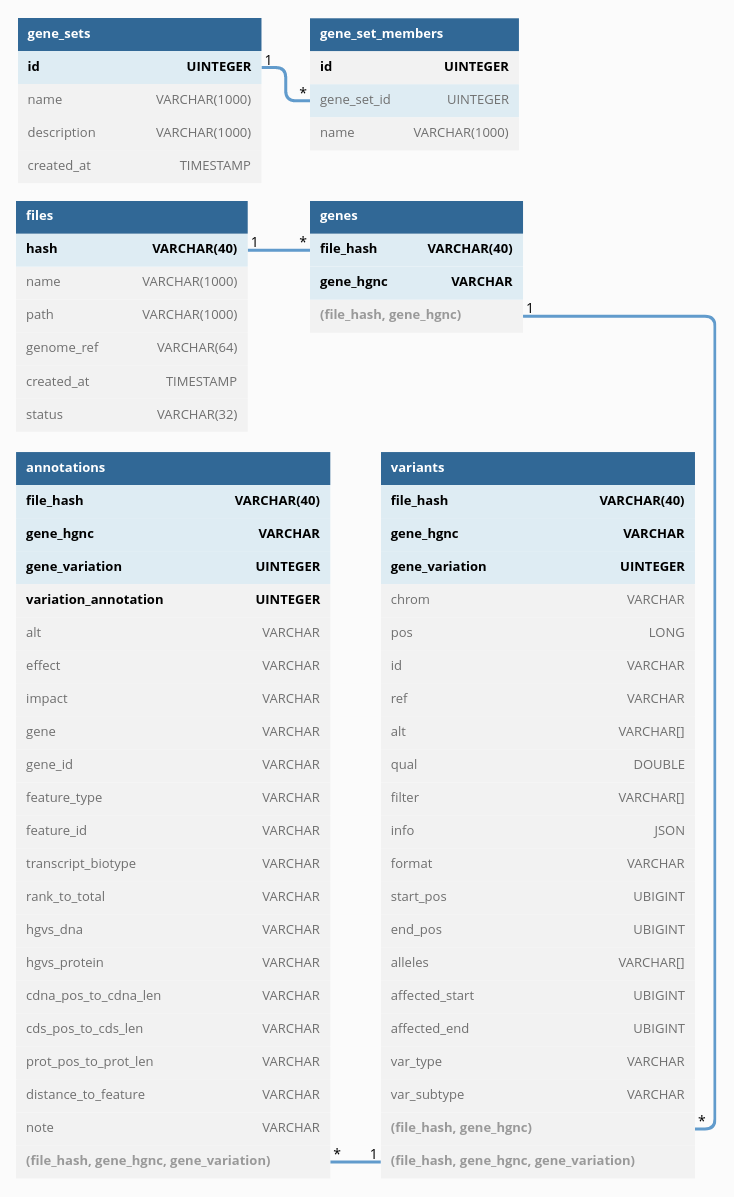
\includegraphics[width=14cm]{figures/db_diagram}
  \caption {Диаграма на структурата на базата данни}
  \label{fig:db_diagram}
\end{figure}

\begin{figure}[h]
  \centering
  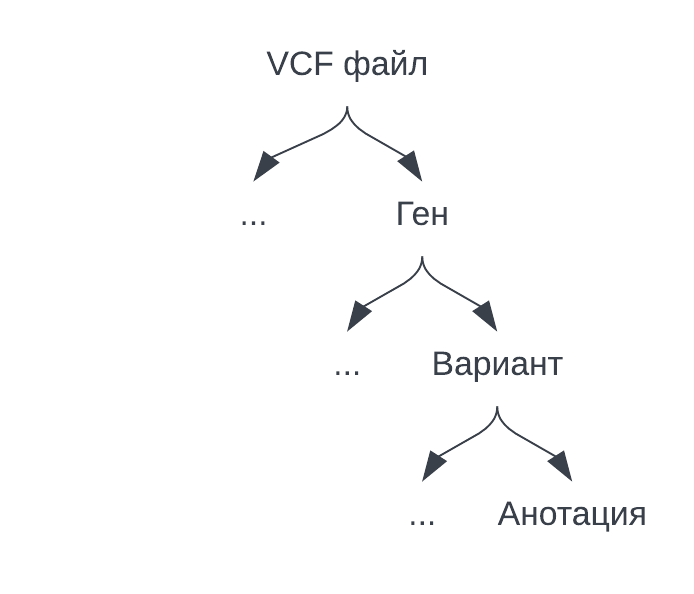
\includegraphics[width=6cm]{figures/annotated_vcf_hierarchy}
  \caption {Йерархично представяне на информацията от анотиран VCF файл}
  \label{fig:annotated_vcf_hierarchy}
\end{figure}


\section{Управление на генни множества}\label{sec:gene_sets}
\paragraph{}
Възможността за управление на генетични множества е проста функционалност, която позволява на потребителя да създава, редактира и изтрива колекции от гени, които представляват цел за някакви изследвания. Всяко генно множество има име, описание и списък от HGNC символи на гени. Дефинирането на генно множество става посредством качване на файл, съдържащ един HGNC символ на ред. В последствие, когато качва VCF файл с генетични множества за обработка, потребителят избира спрямо кое генетично множество да бъде обработен VCF файла. Единствено варианти свързани с гените от това множество ще бъдат запазени в базата данни. Тази, макар и проста функционалност, прави програмното решение по-генерализирано и позволява изследването на различни биологични процеси. Например, ако потребителят качи списък от гени, свързани с ракови заболявания, ще може да изследва полиморфизми за тяхната връзка с рака.

\section{Обработка на VCF при импортиране}
\paragraph{}
Началната точка при работа с разработения софтуер е качване на VCF файл, съдържащ генетични варианти. Това може да бъде направено както с уеб интерфейса, така и с интерфейсът, използваш командния ред (всъщност, импортирането и обработването на VCF е единствената операция, която командния ред може да извършва към момента). При качването на входен VCF файл за обработка, потребителят подава и генно множество, определящо кои гени да бъдат разгледани при обработката (виж секция \ref{sec:gene_sets}).

\paragraph{}
Първата стъпка, която се извършва при обработката на входния VCF е проверка, дали същият файл вече е бил изследван. За целта се калкулира неговата SHA256 хеш сума. Тази сума се използва като главен ключ на таблицата с файлове в базата данни. Ако сумата вече съществува в базата данни, значи файлът вече е бил импортиран и обработката приключва. Ако файлът не е срещан досега, обработката продължава. Прави се валидация, която проверява, че файлът не използва твърде стара версия на VCF стандарта (поддържат се версии не по-малки от 4.0), и се извлича информация за това спрямо кой референтен геном е създаден файлът (фиг. \ref{fig:vcf_processing_sequence}).

\paragraph{}
Следва същинската обработка на входния VCF файл. Първо, външните програми SnpEff и SnpSift, съответно за анотация и филтриране, биват стартирани като отделни процеси. Двата процеса биват свързани посредством pipe оператор, така че анотираните VCF редове, които SnpEff връща, да се подадат директно като входни данни за SnpSift. По този начин SnpEff добавя анотация към редовете на входния VCF, която включва и HGNC символа на гена, с който дадения вариант е свързан. SnpSift филтрира редовете, които му се подават, като оставя само тези, които се отнасят за гени, включени в генното множество, което потребителят е избрал. Резултатът се чете от основната програма, която разглежда всеки ред за да определи за кой ген се отнася и го записва в нов частичен VCF файл, който съдържа само вариантите за дадения ген. Резултатът от тези стъпки е колекция от VCF файлове, всеки от които е анотиран и съдържа само генетичните варианти за един единствен ген. Следващата стъпка е обхождането на всеки от тези файлове, изчитането на данните в Pandas DataFrame обект, който преминава поредица трансформации, и записването на крайната информация в базата данни. Също така, за всеки от тези VCF файлове се създава минимизирана версия, която изключва вариантите определени като незначителни от SnpEff (по-конкретно, за които полето impact има стойност „MODIFIER“). Тази минимизирана версия по-късно се използва за зареждане на генетичните варианти в геномния браузър, като по този начин се осъществява оптимизация на производителността и намаляване на шума за потребителя. Минимизираният и пълният VCF файлове за всеки ген също така се компресират и индексират посредством tabix функционалността (виж секция \ref{sec:samtools_tabix}), предоставяна от модула pysam (виж секция \ref{sec:pysam}). Компресията служи за оптимизация на изискванията към хардуерните ресурси, а създаването на индексни файлове е необходимо за да могат по-късно файловете да се зареждат и визуализират от геномния браузър.

\begin{figure}[htp]
  \centering
  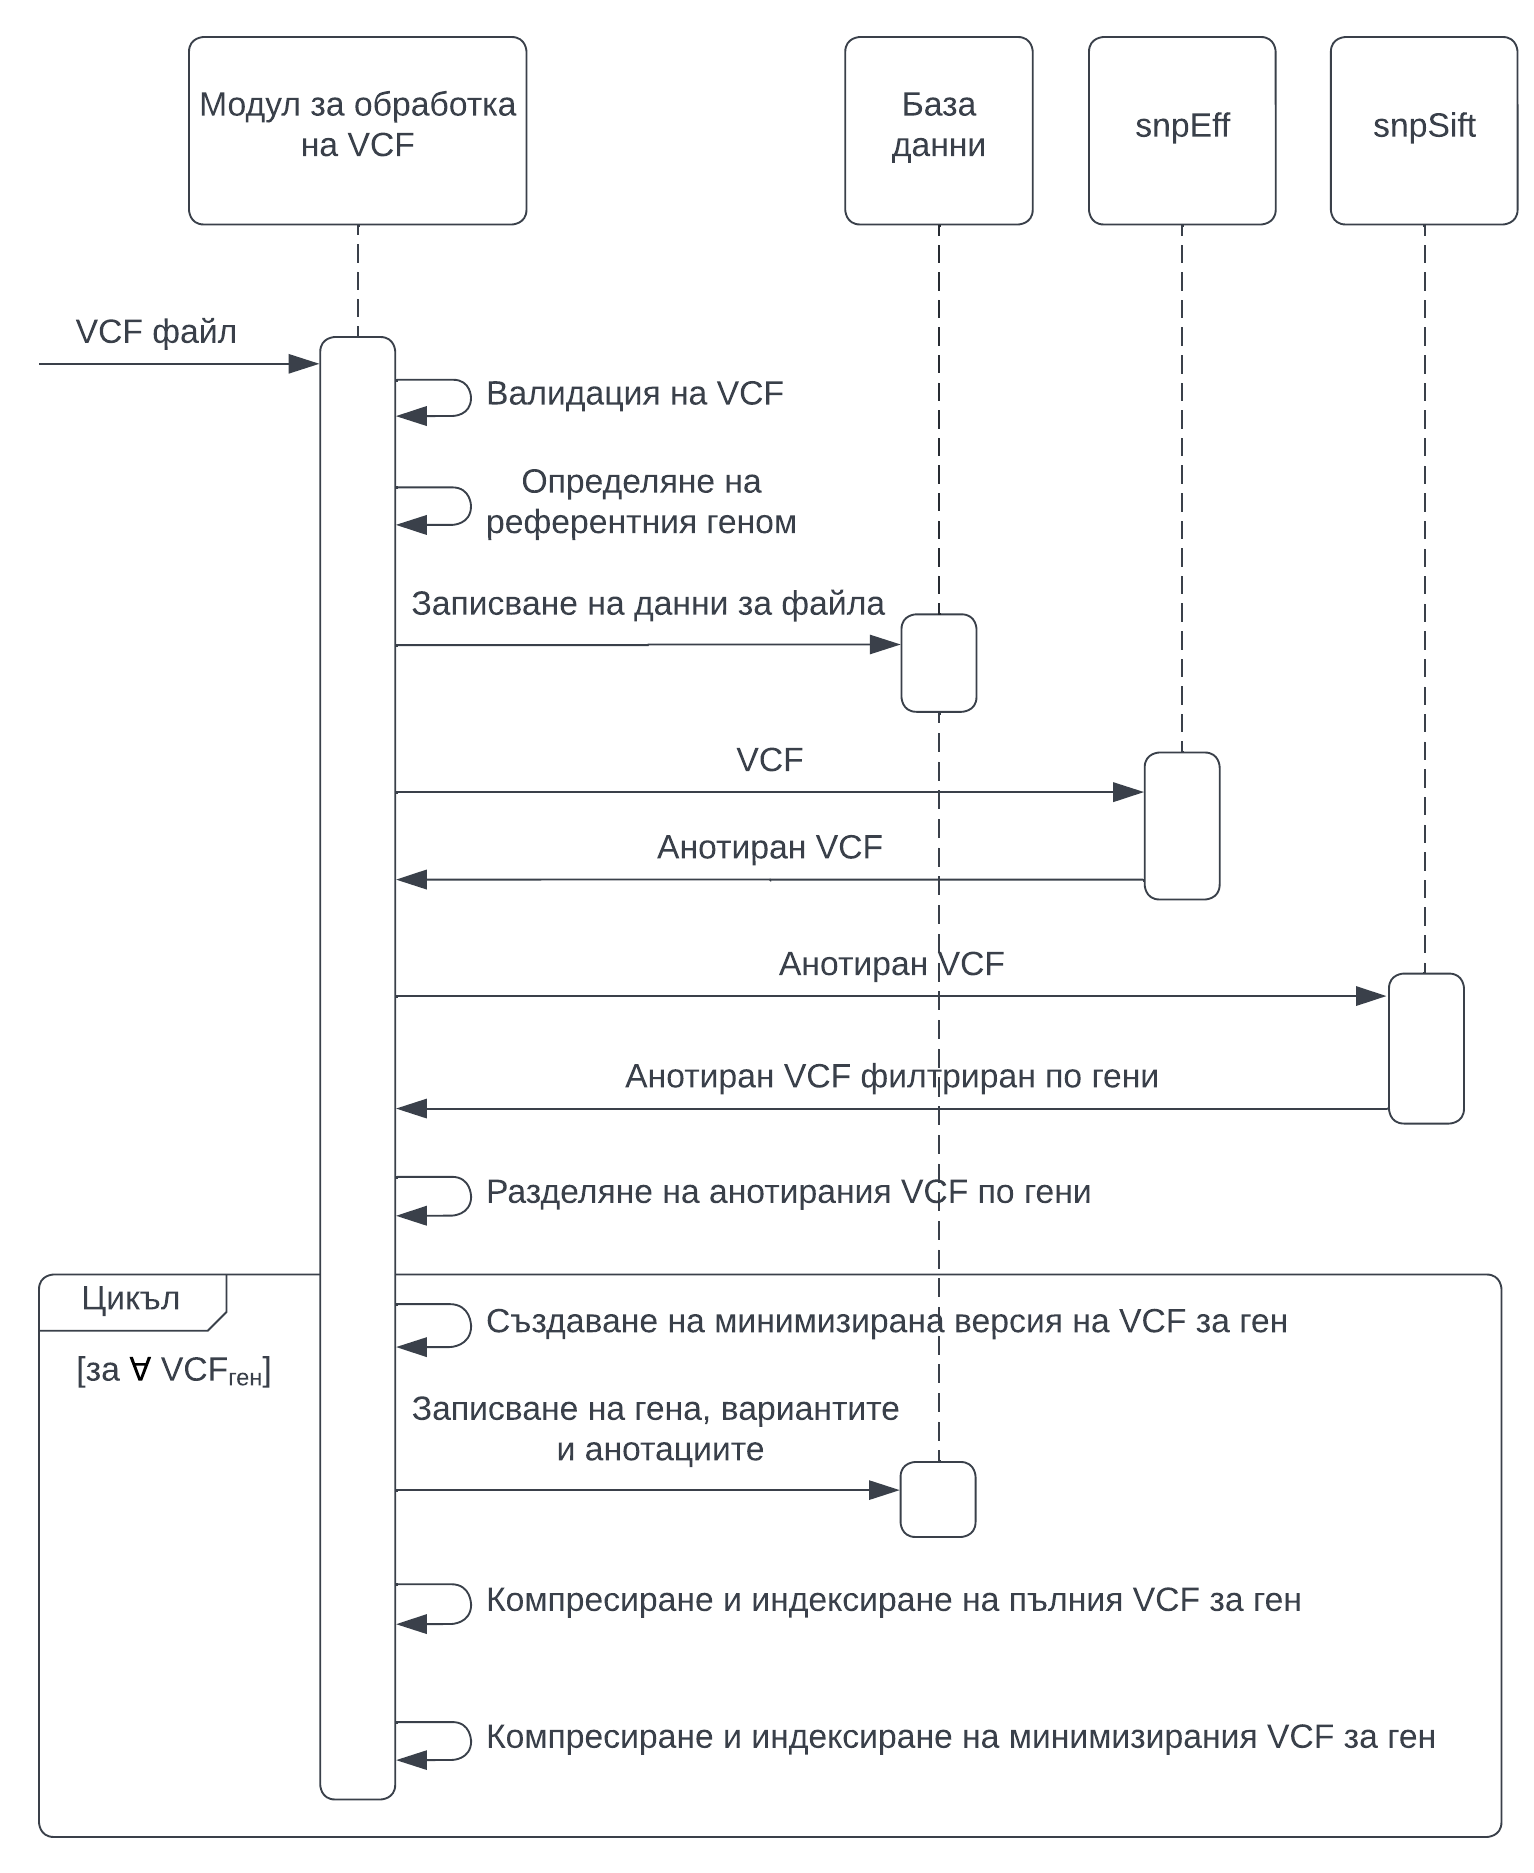
\includegraphics[width=16cm]{figures/vcf_processing_sequence}
  \caption {Диаграма показваща опростено описание на процеса по обработка на VCF файлове с генетични варианти.}
  \label{fig:vcf_processing_sequence}
\end{figure}

\section{Операции върху импортиран VCF}
\paragraph{}
След като един входен VCF, съдържащ генетични варианти, бъде импортиран и обработката му приключи, потребителят може да изследва резултатите. В тази секция са представени основните функции, които програмното решение предоставя.

\subsection{Списък на файлове}
Началната страница предоставя списък с наличните файлове, които вече са импортирани. Потребителят може да избере дали да изследва данните за някой от наличните файлове, да стартира обработката на нов файл или да изтрие информацията за съществуващ файл (фиг. \ref{fig:list_files}).

\subsection{Обзор на файл}
\paragraph{}
Страницата за обзор на файл дава най-обща информация за вече обработен файл. Това включва референтния геном, спрямо който файлът е създаден, генното множество, спрямо което е изследван, броя гени засегнати от полиморфизми и броят анотации. По-детайлна разбивка е дадена в табличен вид, която показва за всеки ген броя варианти и техните анотации спрямо оценената им тежест (фиг. \ref{fig:file_summary}).


\subsection{Обзор на ген}
\paragraph{}
Страницата за обзор на ген дава обща информация за гена и служи като отправна точка за изследването на различните варианти във файла, които го засягат. Страницата предоставя връзки към различни стандартни онлайн бази данни, където потребителят може да открие допълнителна информация за конкретния ген. Тези връзки включват базите данни Ensembl (виж секция \ref{sec:ensembl}), Entrez, HGNC (виж секция \ref{sec:hgnc}) и UniProt. Следва списък от богата анотация за протеина, кодиран от гена, включваща молекулярната функция, процесите и биологичните пътища, в които участва, каталитичната дейност и др (фиг. \ref{fig:gene_summary}). Налична е връзка към страницата, представяща всички варианти за гена.

\paragraph{}
Страницата включва и по-детайлна разбивка на анотираните варианти за гена, представени в табличен вид. Таблицата показва броят на анотациите за варианти, групирани по оценка на тежестта и генетичен ефект. Оценката на тежестта може да е четири варианта: модификатор, ниска, средна, висока. Възможните ефекти са разнообразни и включват например: синонимни мутации, придобиване на стоп кодон, мутации, изменящи смисъла или изместващи рамката, мутации в интрони и др (фиг. \ref{fig:gene_effects}). Всяка от стойностите в таблицата представлява връзка, при натискането на която, потребителят бива препратен към страницата за варианти, като се добавя филтър за конкретната стойност, така че потребителят да може да разгледа точно този вид варианти.

\subsection{Варианти на ген}
\paragraph{}
В страницата за варианти да ген потребителят има достъп до геномен браузър, чрез който може да изследва полиморфизмите засягащи гена. При отварянето на страницата, браузърът автоматично се фокусира върху геномния регион, съдържащ списъка от варианти във VCF файла. Геномният браузър представя няколко различни информационни ленти. Първата лента показва генните варианти. Тъй като VCF файлът може да е за един експеримент, или множество експерименти, тази лента показва също така и комбинациите от изразени варианти за всеки от експериментите във VCF файла. Втората лента показва гените, като са обособени техните екзони и интрони. Третата лента показва транскриптите, които се кодират от даден ген, заедно с техните Ensembl идентификатори (фиг. \ref{fig:genome_browser}).

\paragraph{}
В страницата също е налична странирана таблица с всички варианти за гена. Таблицата представя началната и крайната точка на полиморфизма, референтната и алтернативната нуклеотидна поредица, типа и подтипа на полиморфизма (точкова мутация, вмъкване, изтриване и тн.). Налични са и контроли, с които могат да бъдат прилагани сложни филтри върху данните от таблицата (фиг. \ref{fig:variants_list}).

\subsection{Засегнати транскрипти}
\paragraph{}
За всеки генетичен вариант можем да достъпим страница със засегнатите от него транскрипти. Страницата предоставя таблица с Ensembl идентификатора на транскрипта, неговия тип (например протеинокодиращ, псевдоген и тн), ефекта, който полиморфизма оказва върху този транскрипт, тежеста на промяната и HGVS номенклатура (виж секция \ref{sec:hgvs}) на промяната на протеина, ако има такава. Потребителят също така може да сравни и референтния и алтернативния протеин за този транскрипт (фиг. \ref{fig:protein_comparison}).

\chapter{Дискусия}
\chapter{Изводи}


\bibliographystyle{plain}
\bibliography{refs}
\addcontentsline{toc}{chapter}{Библиография}

\chapter{Приложение}

\begin{figure}[h]
  \centering
  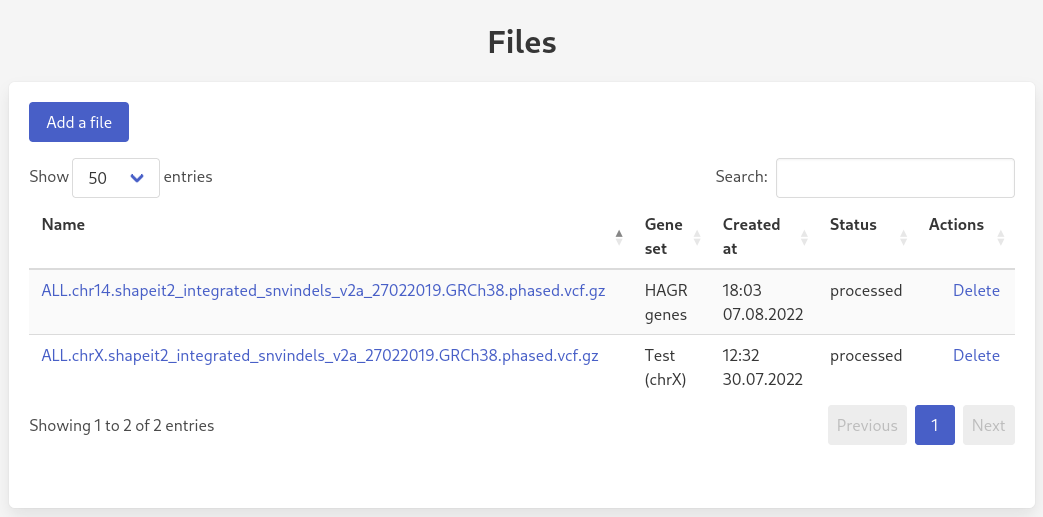
\includegraphics[width=16cm]{figures/list_files}
  \caption {Списък от файлове.}
  \label{fig:list_files}
\end{figure}


\begin{figure}[ht]
  \centering
  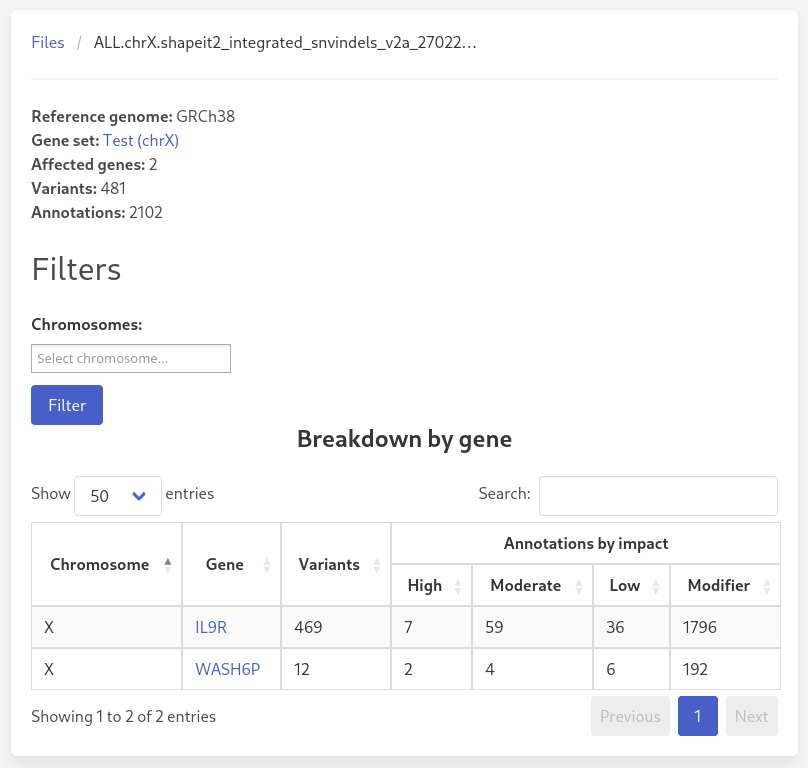
\includegraphics[width=16cm]{figures/file_summary}
  \caption {Обзор на файл.}
  \label{fig:file_summary}
\end{figure}

\begin{figure}[ht]
  \centering
  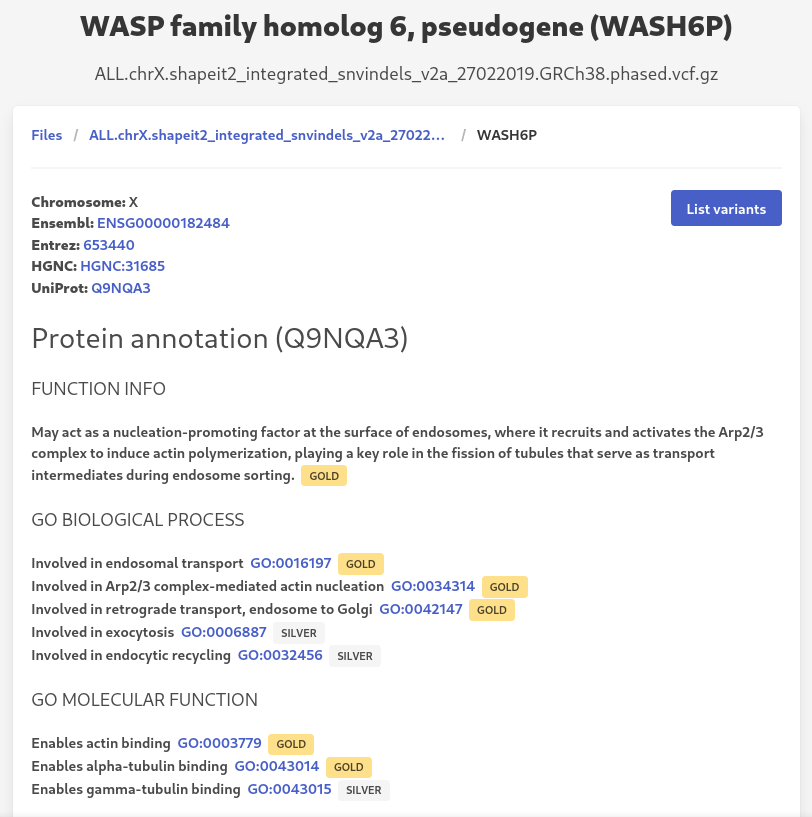
\includegraphics[width=16cm]{figures/gene_summary}
  \caption {Обща информация за гена.}
  \label{fig:gene_summary}
\end{figure}

\begin{figure}[ht]
  \centering
  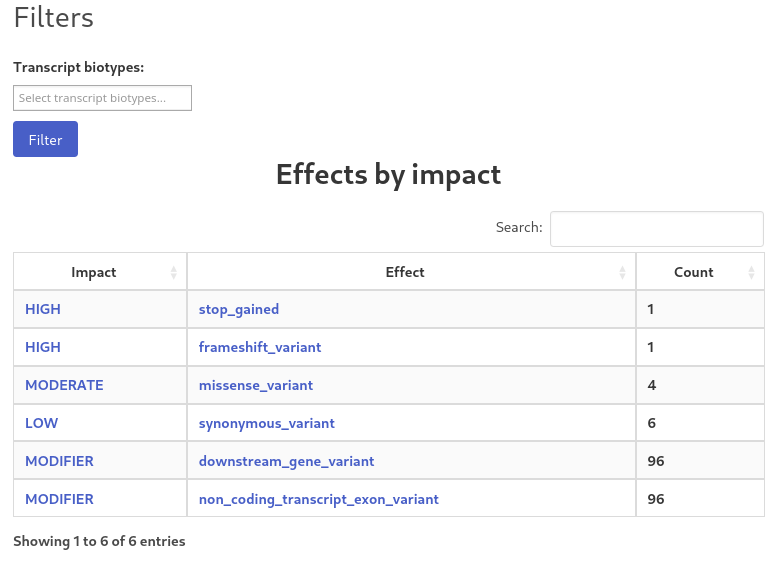
\includegraphics[width=16cm]{figures/gene_summary_effects}
  \caption {Разбивка на анотираните варианти и техните предсказани ефекти.}
  \label{fig:gene_effects}
\end{figure}

\begin{figure}[ht]
  \centering
  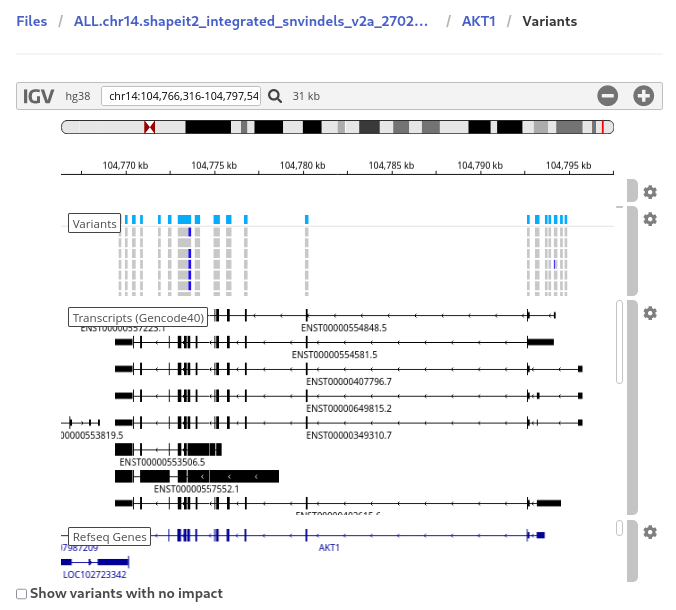
\includegraphics[width=16cm]{figures/genome_browser}
  \caption {Геномен браузър за изследване на генетичните варианти.}
  \label{fig:genome_browser}
\end{figure}

\begin{figure}[ht]
  \centering
  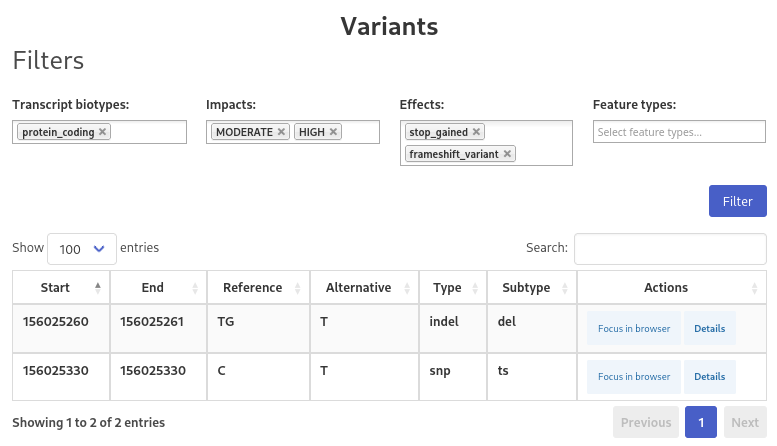
\includegraphics[width=16cm]{figures/variants_list}
  \caption {Таблица с геномни варианти и филтри.}
  \label{fig:variants_list}
\end{figure}

\begin{figure}[ht]
  \centering
  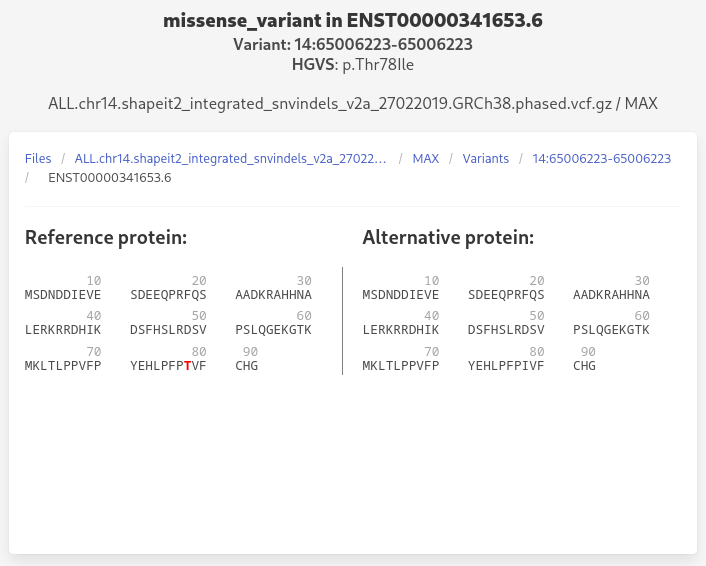
\includegraphics[width=16cm]{figures/protein_comparison}
  \caption {Сравнение на референтен и алтернативен протеин. Мястото на полиморфизма е оцветено в червено.}
  \label{fig:protein_comparison}
\end{figure}

\end{document}